
%%%%%%%%%%%%%%%%%%%%%%%%%%%%%%%%%%%%%%%%%%%%%%%%%%%%%%%%%%%%%%%%%%%%%%%%%%%%%%%%
%%%%%%%%%%%%%%%%%%%%%%%%%%%%%%%%%%%%%%%%%%%%%%%%%%%%%%%%%%%%%%%%%%%%%%%%%%%%%%%%
\section{Exemplos de treinamentos cognitivo-motor multicomponente}

Os exemplos presentados a continuação trabalham três componentes necessários na dança,
estes são:
\begin{itemize}
\item A \hyperref[cap:percepcaomusical]{\textbf{percepção musical}}: 
neste caso serão trabalhadas a \hyperref[sec:percepcionmetrica]{\textbf{percepção da métrica}} 
e/ou \hyperref[sec:perceberfrases]{\textbf{das frases musicais}}, 
as quais podem ser extraídas de uma música ou de algum ritmo simples gerado digitalmente.
\item O \hyperref[sec:BodyControl]{\textbf{controle corporal}}: 
no qual executaremos um movimento ou passo de dança que estará subordinado
à métrica escolhida no item anterior.
\item A atividade externa: representada por um objeto ou atividade
as quais devemos comandar ou conduzir seguindo a métrica escolhida.
\end{itemize}

\begin{example}[Treino cognitivo-motor multicomponente com movimentos simples:]
\label{ex:treino-cognitivo-multi-simples}
Como é mostrado na Tabela \ref{tab:treino-bolinha1}, 
neste exercício devemos escolher trés componentes distintos os quais executaremos de forma simultânea.
\begin{itemize}
\item A primeira escolha corresponde ao ritmo que seguiremos em nosso treinamento, 
este pode ser 
um ``tchic tchic tum'', \meter{2}{4}\leftrepeat~\Vier\Acht\Acht~\rightrepeat, ou 
um ``tum tum'', \meter{2}{4}\leftrepeat~\Vier\Vier~\rightrepeat, 
em qualquer destes dois casos um ``tum'' deve coincidir com o \hyperref[subsec:perceberTF1]{\textbf{tempo forte}}.
A fonte de informação musical pode vir de
    \begin{itemize}
    \item uma música em compasso binário, ex: ``Suingue de Samba'' interpretado por Rogê (ritmo 2), ou de 
    \item um metrônomo (ritmo 1).
    \end{itemize}
Neste caso o importante é souber \hyperref[subsec:perceberTF1]{\textbf{reconhecer o tempo forte}}.
\item A segunda escolha corresponde ao movimento a ser realizado, os quais podem ser:
    \begin{itemize}
    \item caminhadas ou balanços se o ritmo escolhido é ``tum tum'', e
    \item caminhadas, básicos frente trás ou cruzados se nosso ritmo escolhido é um ``tchic tchic tum''.
    \end{itemize}
Em ambos casos realizaremos uma pisada com troca de peso do corpo por cada figura musical.
\item A terceira escolha é a atividade externa, a qual podem ser: 
    \begin{itemize}
    \item jogar uma bolinha ao ar e pegar-lha novamente exatamente quando se escute o tempo forte (atividade 1), ou podemos 
    \item jogar uma bolinha ao chão de modo que esta rebote no exato momento em que se escute o tempo forte (atividade 2).
    \end{itemize}
\end{itemize}
\end{example}

\begin{table}[!h]
  \centering
    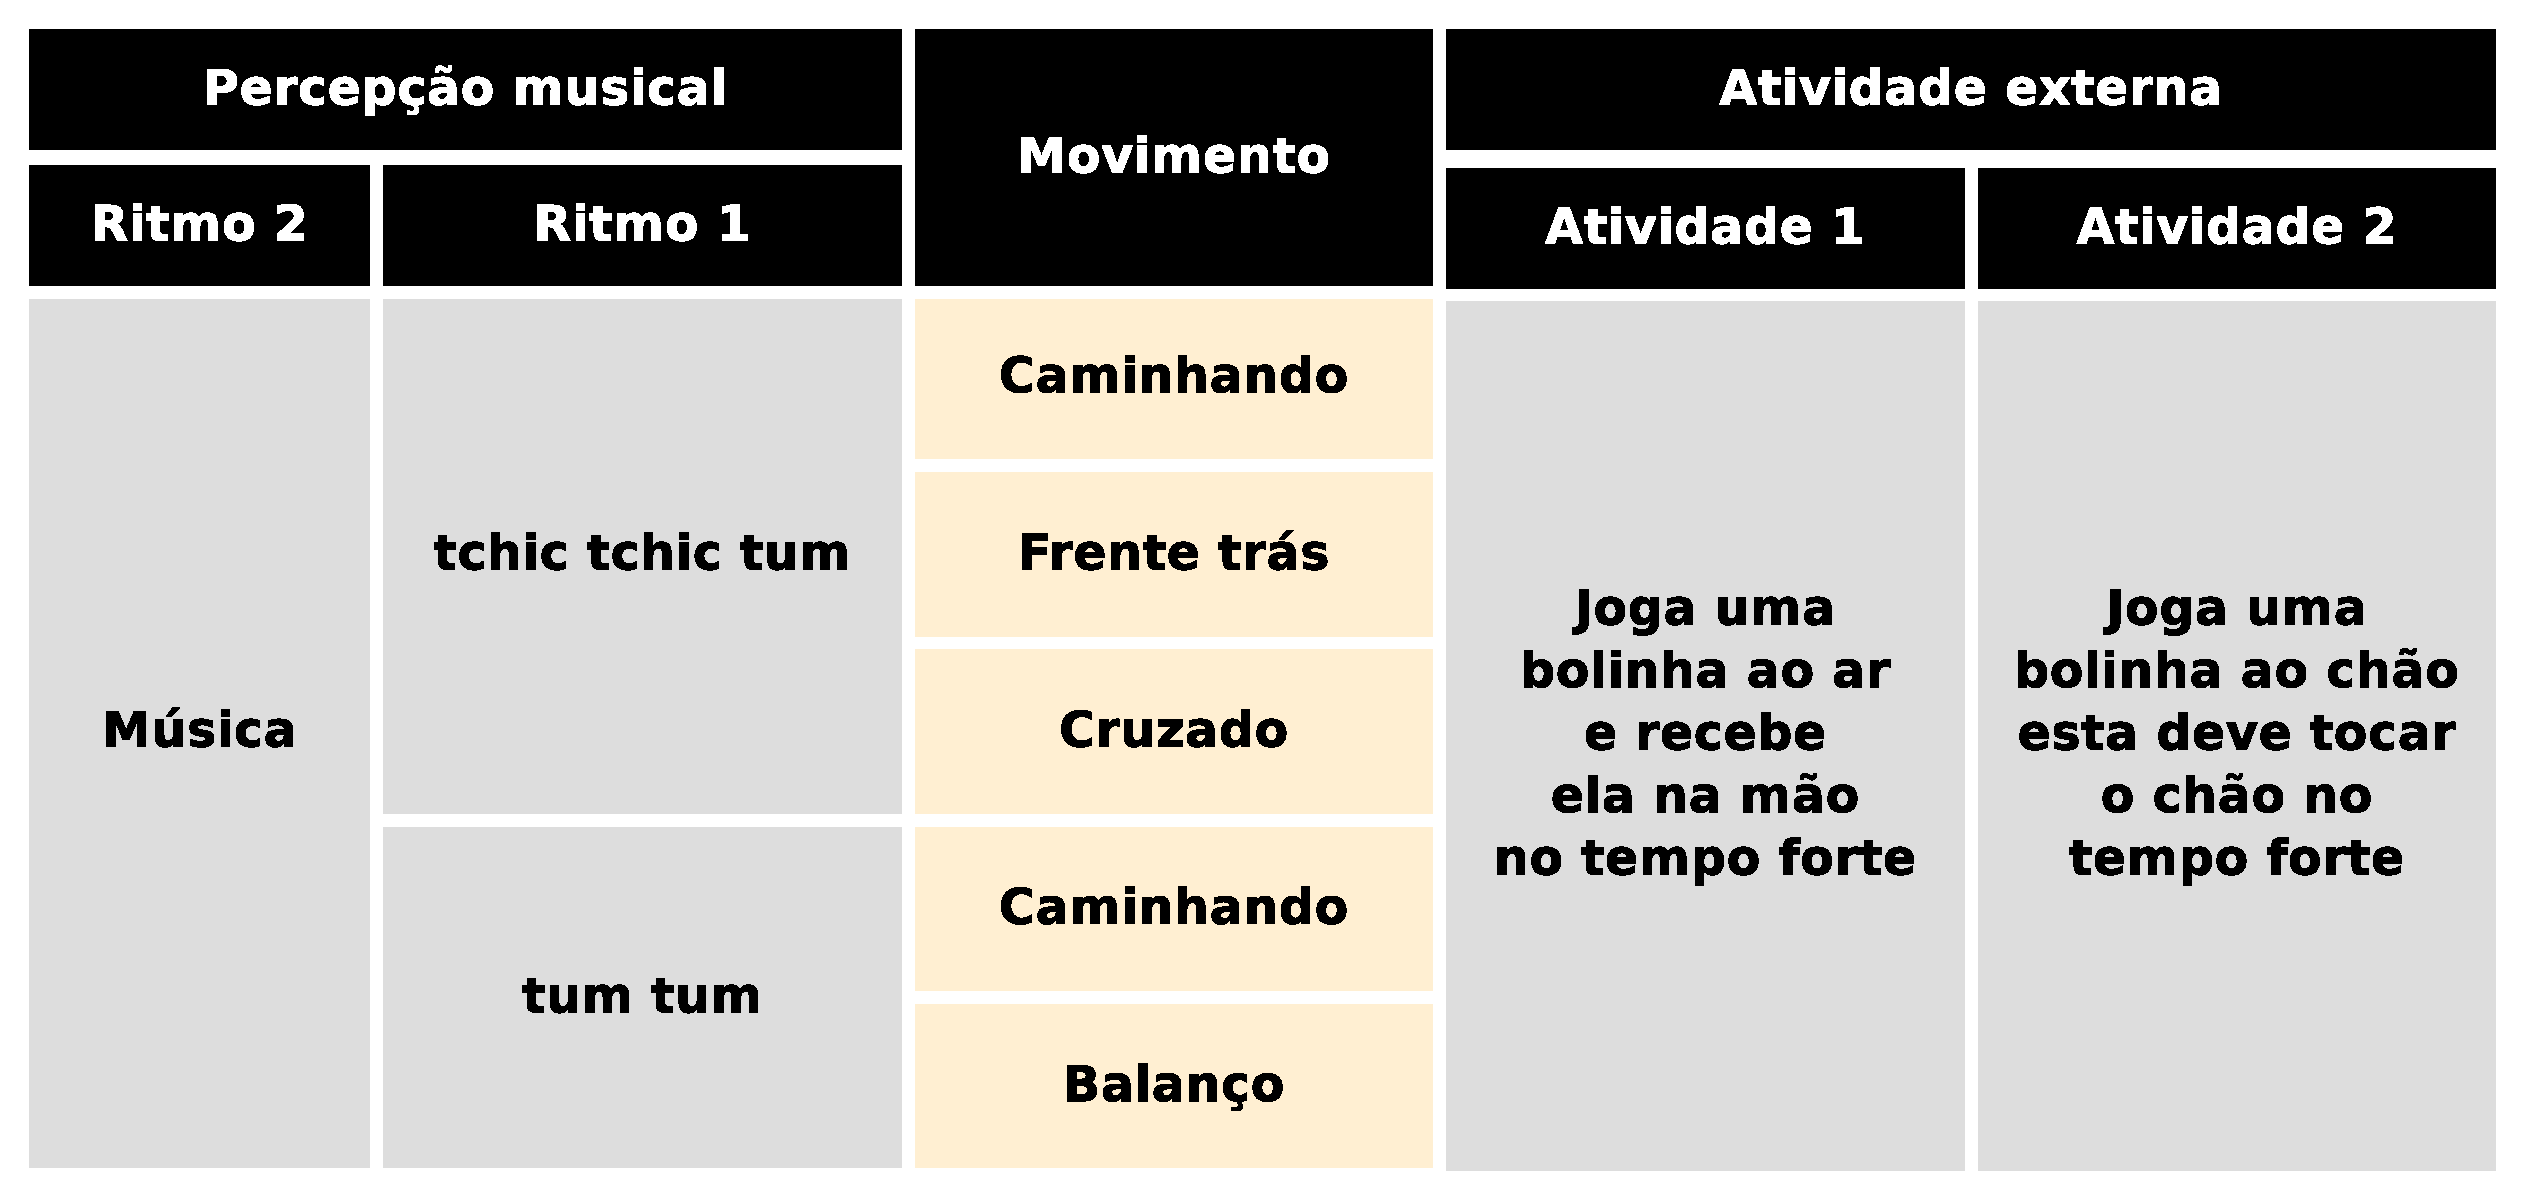
\includegraphics[width=1.0\textwidth]{chapters/cap-body-control/treino-bolinha1.eps}
\caption{Treino cognitivo-motor multicomponente com movimentos simples.}
\label{tab:treino-bolinha1}
\end{table}


Se o Exemplo \ref{ex:treino-cognitivo-multi-simples} resulta simples de seguir, 
pode ser interessante pausar aleatoriamente no meio da música e 
aprender a voltar corretamente na métrica,
até que consigamos \hyperref[subsec:perceberTF1]{\textbf{reconhecer de forma fácil o tempo forte}}.
Com essas pausas evitamos que nosso cérebro crie um atalho,
e só identifique o tempo forte do primeiro compasso, e 
logo só conte os segundos até o próximo tempo forte.
%A ideia do exercício é ganhar a habilidade de voltar a pegar facilmente a 
%métrica da música após algum erro ou pausa na dança.



\begin{example}[Treino cognitivo-motor multicomponente com movimentos complexos:]
Este exemplo é similar ao Exemplo \ref{ex:treino-cognitivo-multi-simples}
no qual são trabalhadas em simultâneo trés componentes da dança,
com a diferença de que aqui só é usado o ritmo ``tchic tchic tum'', 
\meter{2}{4}\leftrepeat~\Vier\Acht\Acht~\rightrepeat,
o qual pode vir de: 
    \begin{itemize}
    \item uma música em compasso binário, ex: ``Piston de Gafieira'' interpretado por Toquinho (ritmo 2), ou de 
    \item um metrônomo (ritmo 1).
    \end{itemize}
Como mostra a Tabela \ref{tab:treino-bolinha2}, 
os movimentos que podemos escolher são um pouco mais complexos,
tais como a trança, escovinha, etc. 
e devem ser executados mediante uma troca de peso do corpo por cada figura musical.
Finalmente, as possíveis atividades externas são as mesmas que no 
Exemplo \ref{ex:treino-cognitivo-multi-simples}
\end{example}

\begin{table}[!h]
  \centering
    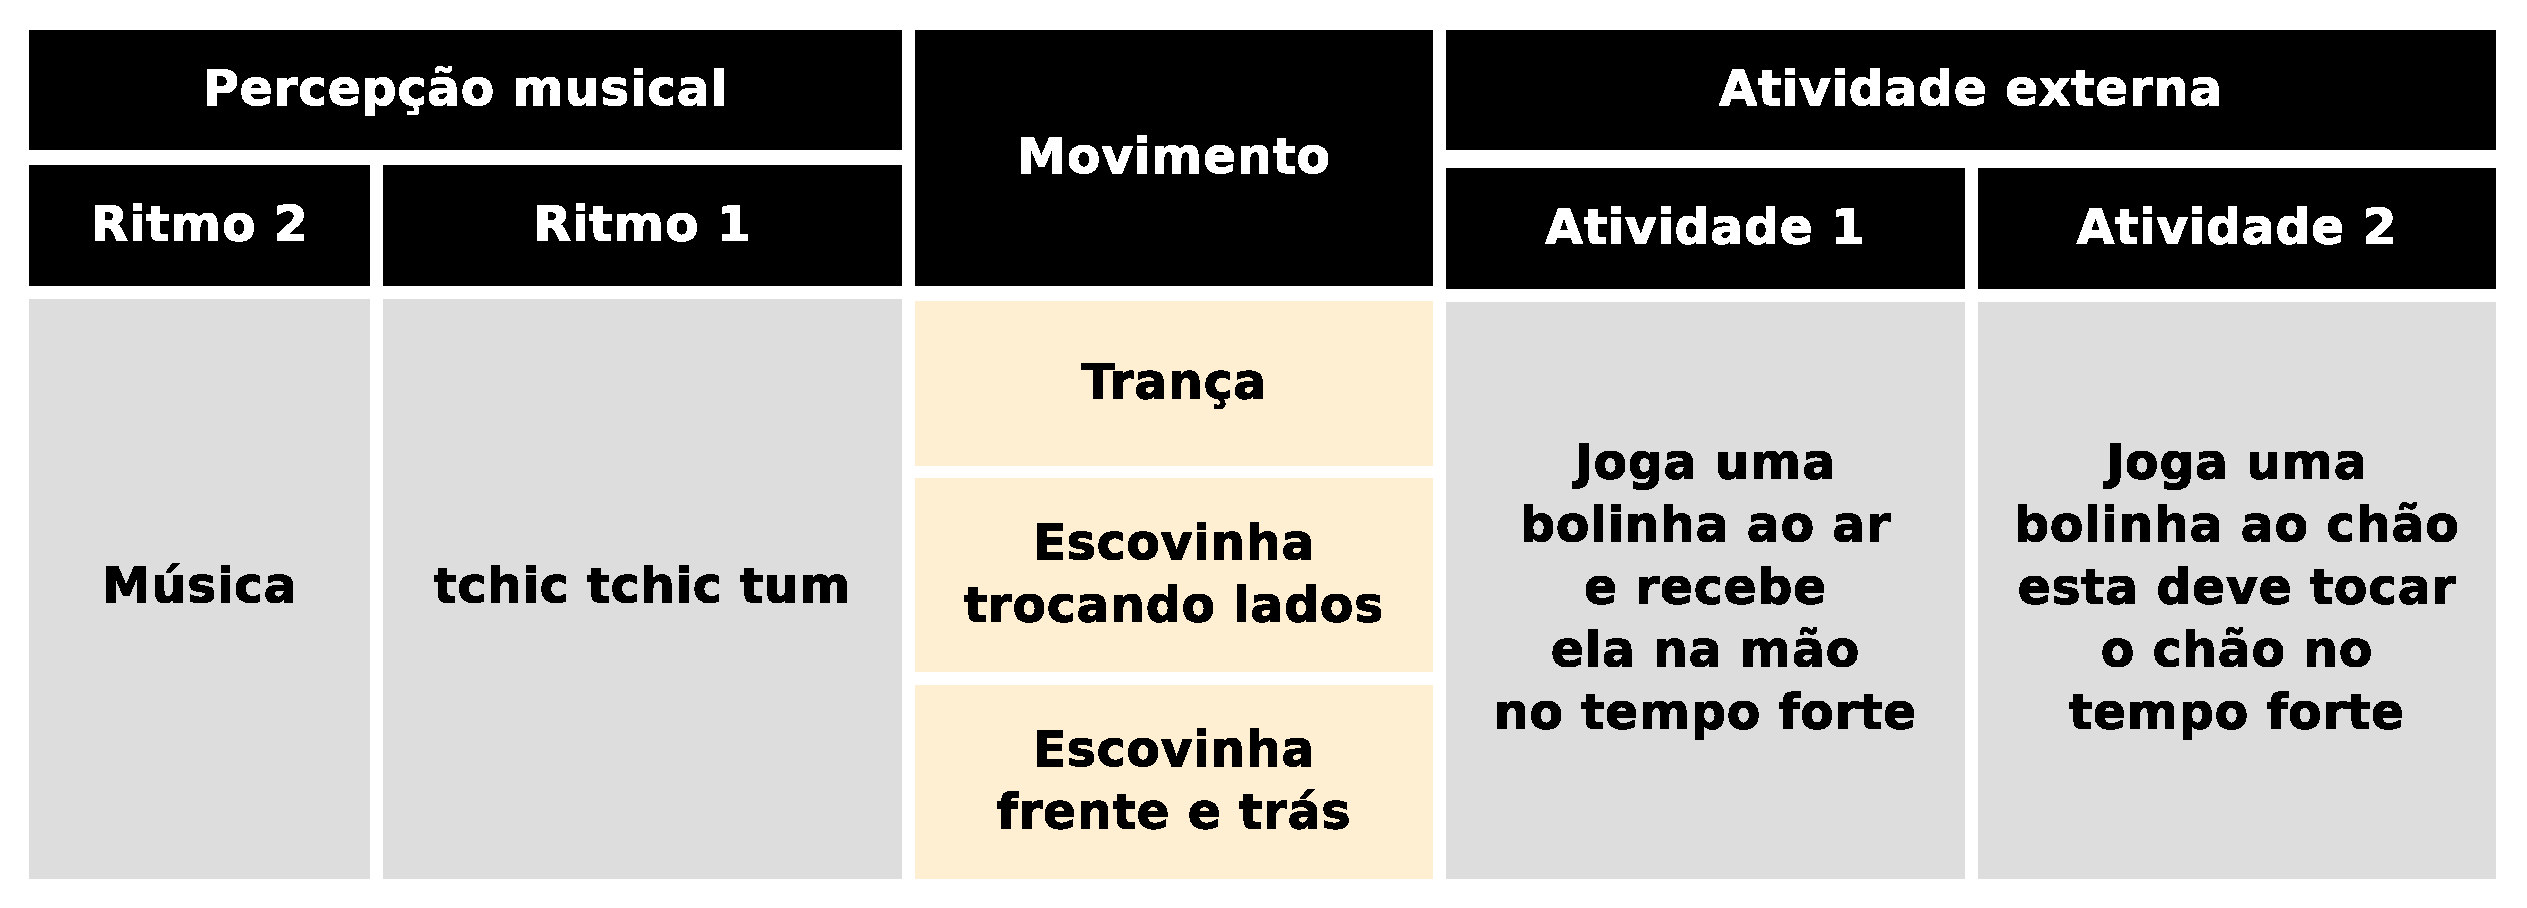
\includegraphics[width=1.0\textwidth]{chapters/cap-body-control/treino-bolinha2.eps}
\caption{Treino cognitivo-motor multicomponente com movimentos complexos.}
\label{tab:treino-bolinha2}
\end{table}

A seguir são mostrados alguns exemplos de treino cognitivo-motor multicomponente 
que ajudaram a explorar nosso controle corporal e a percepção das frases na música.

\begin{example}[Treino cognitivo-motor multicomponente relativo à percepção do final de frase musical:]
Como é mostrado na Tabela \ref{tab:treino-bolinha3},
neste exercício devemos escolher trés componentes distintas que serão executadas de forma simultânea.
\begin{itemize}
\item Na primeira escolha temos a percepção musical do 
\hyperref[pos:detetandoiniciofrase]{\textbf{final de frase musical}} 
e do último tempo forte da frase, na qual a fonte de informação musical pode vir de:
    \begin{itemize}
    \item uma música em compasso binário, ex: ``Cabide'' interpretado por Ana Carolina e Luiz Melodia (ritmo 2), ou
    \item um ritmo gerado de forma sintética (ritmo 1),
    ex: a melodia ``lamento e consolo'' mostrada na Figura \ref{fig:lamento-e-consolo}, 
    na qual todas as frases musicais finalizam no tempo forte.
    \end{itemize}
Neste caso o objetivo é usar uma música que nos permita treinar
como \hyperref[pos:detetandoiniciofrase]{\textbf{reconhecer o final de frase musical}}. 
É importante lembrar que as frases musicais podem ter um 
\hyperref[subsec:finaldefrasemus1]{\textbf{final masculino ou feminino}}, 
porém nos estamos interessados em reconhecer o ultimo tempo forte.
\item A segunda escolha corresponde ao movimento a ser realizado,
neste caso podemos usar:
    \begin{itemize}
    \item caminhadas ou balanços seguindo um ritmo ``tum tum'', 
    \meter{2}{4}\leftrepeat~\Vier\Vier~\rightrepeat, ou 
    \item caminhadas, básicos frente trás ou cruzados seguindo um ritmo ``tchic tchic tum'', 
    \meter{2}{4}\leftrepeat~\Vier\Acht\Acht~\rightrepeat.
    \end{itemize}
Em ambos casos realizaremos uma pisada com troca de peso do corpo por cada figura musical.
\item A terceira escolha é a atividade externa, as quais podem ser: 
    \begin{itemize}
    \item jogar uma bolinha ao ar e pegar-lha novamente exatamente no último tempo forte da cada frase musical (atividade 1), ou
    \item podemos jogar a bolinha ao chão de modo que rebote no último tempo forte da cada frase musical (atividade 2).
    \end{itemize}
\end{itemize}
\end{example}

\begin{table}[!h]
  \centering
    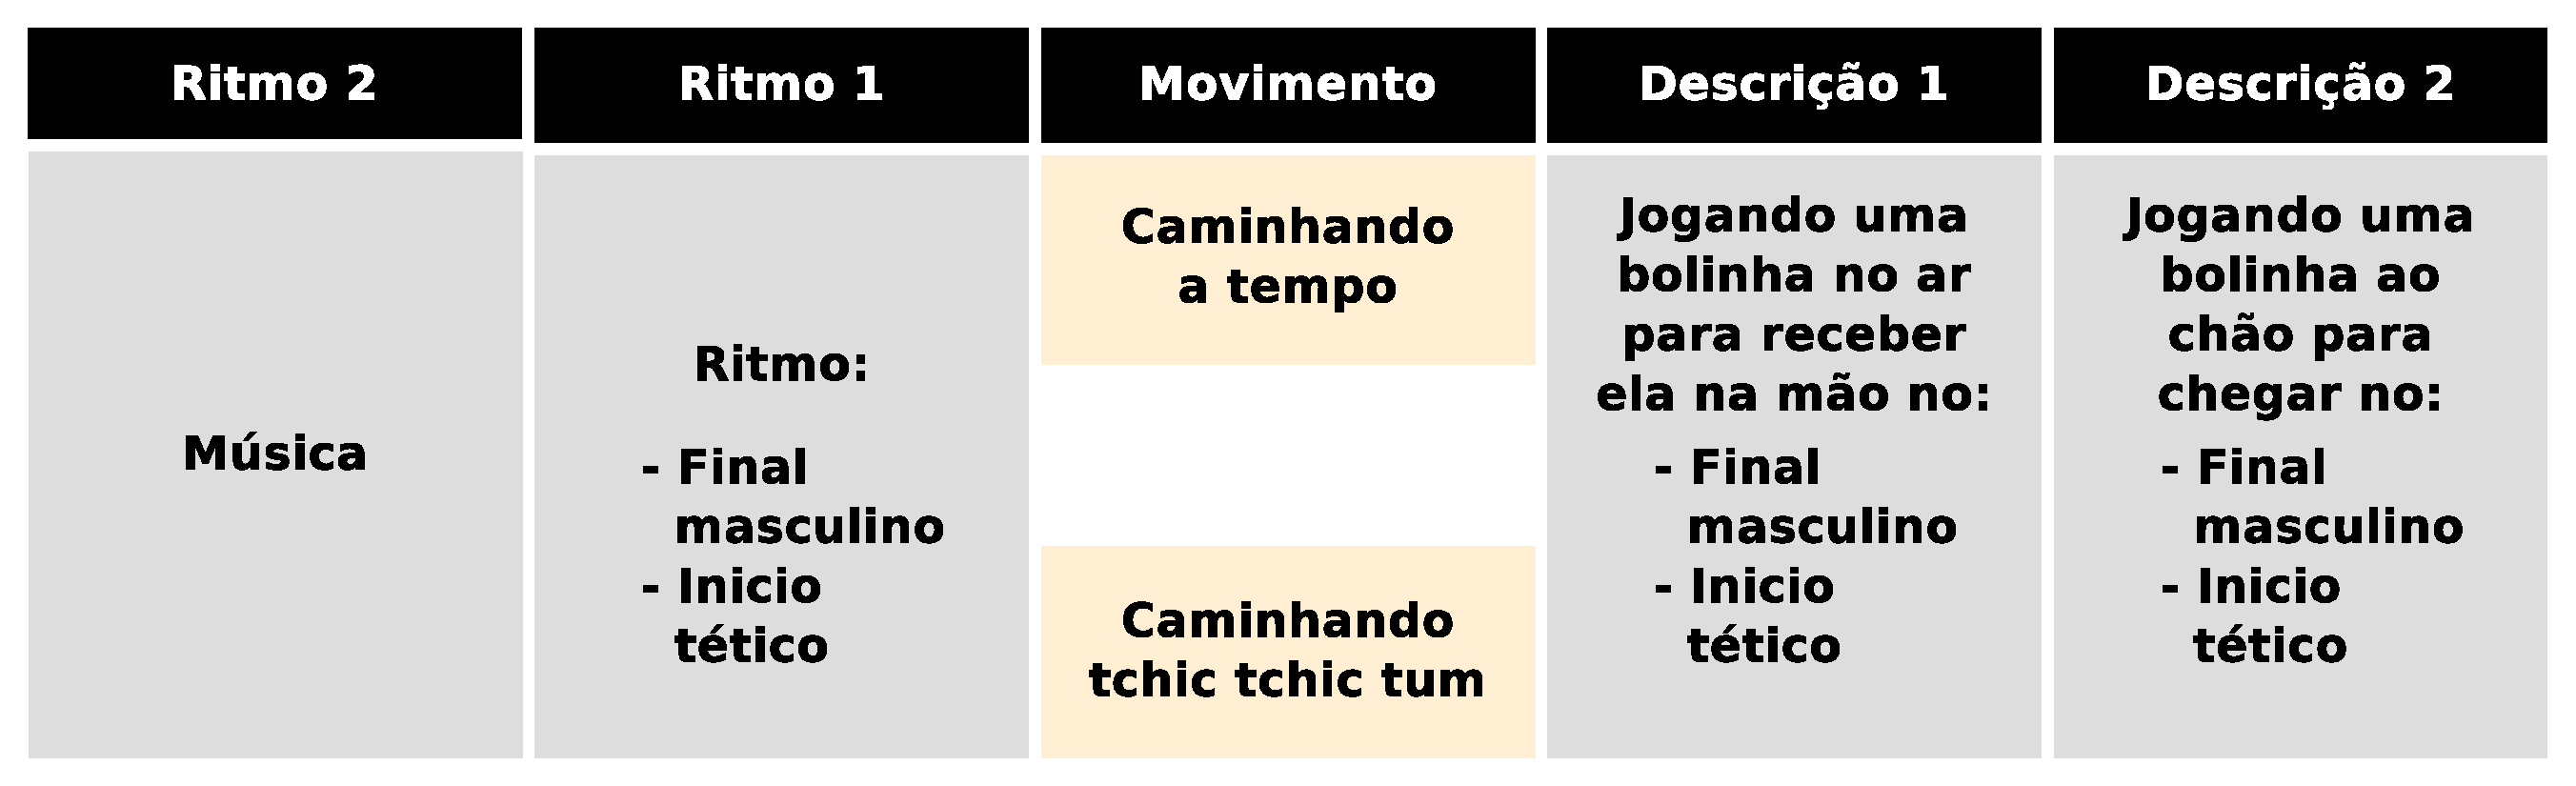
\includegraphics[width=1.0\textwidth]{chapters/cap-body-control/treino-bolinha3.eps}
\caption{Treino cognitivo-motor multicomponente relativo à percepção do final de frase musical.}
\label{tab:treino-bolinha3}
\end{table}



\begin{example}[Treino cognitivo-motor multicomponente relativo à percepção do inicio da frase musical:]
Como é mostrado na Tabela \ref{tab:treino-bolinha4},
neste exercício devemos escolher trés componentes que executaremos em simultâneo.
\begin{itemize}
\item A primeira escolha corresponde à percepção do \hyperref[pos:detetandoiniciofrase]{\textbf{inicio da frase musical}},
especificamente procuramos reconhecer o primeiro tempo forte da frase.
A fonte de informação musical pode vir de:
    \begin{itemize}
    \item uma música em compasso binário, ex: ``Tamborim'' interpretado pelo Clube do Balanço (ritmo 2) 
    o qual tem frases de 4 compassos fáceis de identificar, ou de
    \item um ritmo gerado de forma sintética (ritmo 1),
    ex: a melodia ``lamento e consolo'' mostrada na Figura \ref{fig:lamento-e-consolo}, 
    na qual todas as frases musicais tem um \hyperref[subsec:InicioFraseMusical]{\textbf{ritmo anacrústico}}
    fácil de acompanhar.
    \end{itemize}
Neste caso o importante é escolher uma música que nos permita treinar
como \hyperref[pos:detetandoiniciofrase]{\textbf{reconhecer o inicio da frase musical}}
e o primeiro tempo forte da frase. 
É importante lembrar que as frases musicais podem ter um inicio com 
\hyperref[subsec:InicioFraseMusical]{\textbf{ritmo tético, anacrústico ou acéfalo}}.
\item A segunda escolha que devemos fazer é o movimento a ser realizado,
neste caso podemos usar:
    \begin{itemize}
    \item caminhadas ou balanços em tempo, quer dizer seguindo um ritmo ``tum tum'', 
    \meter{2}{4}\leftrepeat~\Vier\Vier~\rightrepeat, e
    \item caminhadas, básicos frente trás ou cruzados seguindo um ritmo ``tchic tchic tum'', 
    \meter{2}{4}\leftrepeat~\Vier\Acht\Acht~\rightrepeat.
    \end{itemize}
Em ambos casos realizaremos uma pisada com troca de peso por cada figura musical.
\item A terceira escolha é a atividade externa, a qual pode ser: 
    \begin{itemize}
    \item mudar a direção de nosso movimento no primeiro tempo forte de cada frase musical (atividade 1), ou
    \item podemos jogar a bolinha ao chão de modo que rebote no último tempo forte da cada frase musical (atividade 2).
    \end{itemize}
\end{itemize}
\end{example}

\begin{table}[!h]
  \centering
    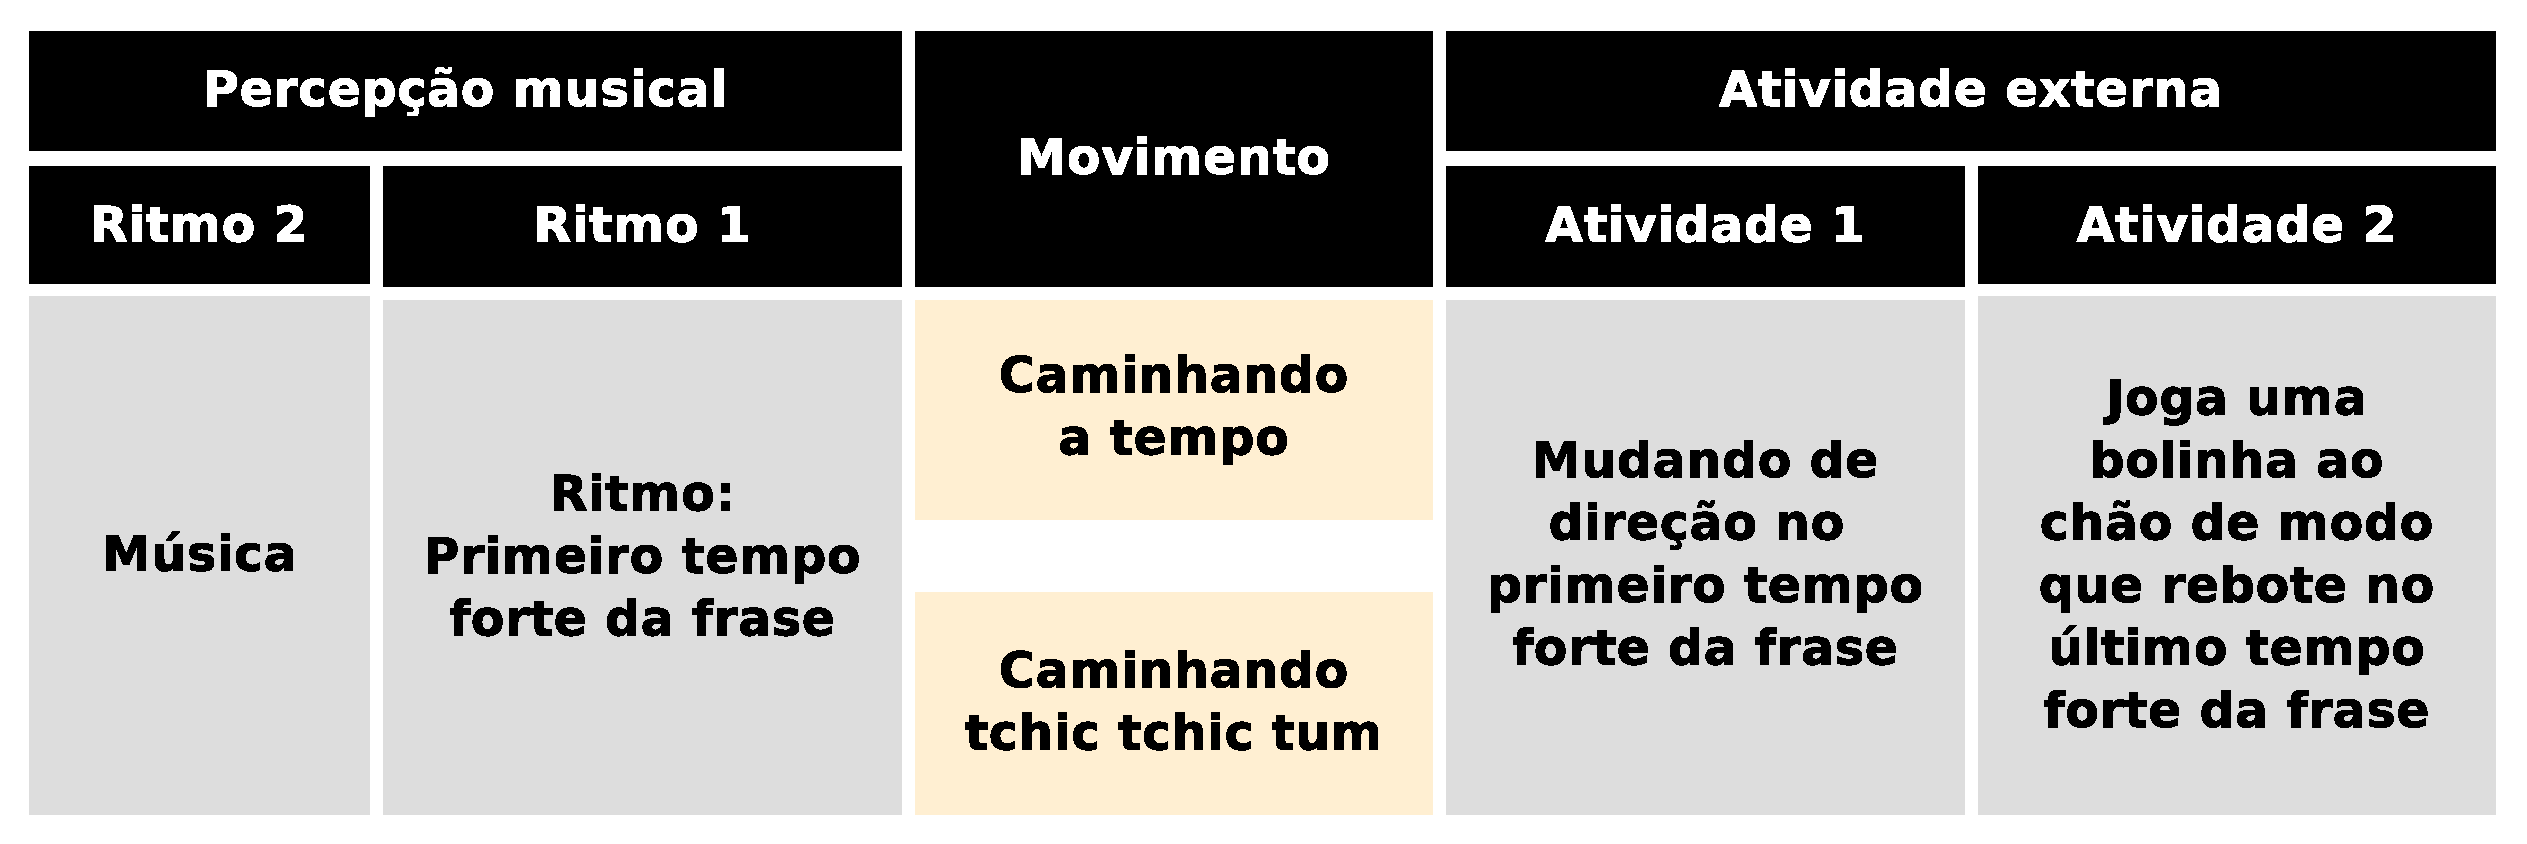
\includegraphics[width=1.0\textwidth]{chapters/cap-body-control/treino-bolinha4.eps}
\caption{Treino cognitivo-motor multicomponente relativo à percepção do inicio da frase musical.}
\label{tab:treino-bolinha4}
\end{table}


%\section{\textcolor{red}{  Treino de ombros no plano frontal}}
%\section{\textcolor{red}{  Treino do quadril no plano frontal}}

